\chapter{Solution}
Our solution consists of a general protocol, which fulfills the demands of the proposed network outlined in 1.2 Purpose and solves the underlying problem described in 1.3 Problem.
In addition to the protocol, a reference implementation has been developed and tested on a small scale network.

\section{General protocol}
The network connects clients, who pay to perform work, with workers, that get paid to perform work. In order for the network, and its cloud computing platform, to thrive, it relies on an open market where the supply of workers meets the demand of clients. Any person with a computer could register to become a worker and get paid for the work they perform, and conversely, any person with the desire to execute arbitrary code can do so, provided they can pay for it. The high level flow of workers and clients within the network is shown in figure~\ref{network-schema}.

\begin{figure}[ht]
\centering
\begin{tikzpicture}[auto]
   \node[cloud, cloud puffs=15.7, cloud ignores aspect, minimum width=4cm, minimum height=2cm, draw, align=center] (butt) {Network}; 
   \node[ellipse,draw] (cli)  [left=of butt]        {Client}; 
   \node[ellipse,draw] (wkr1) [right=of butt]       {Worker}; 
   \node[ellipse,draw] (wkr2) [below right=of butt] {Worker}; 
   \node[ellipse,draw] (wkr3) [below left=of butt]  {Worker}; 
    \path[-latex] 
    (cli)   edge              node        {2} (butt)
    (wkr1)  edge              node [swap] {1} (butt)
    (wkr2)  edge [bend left]  node [swap] {1} (butt)
            edge [loop right, ->, >=latex] node {4} (wkr2)
    (wkr3)  edge              node        {1} (butt)
    (butt)  edge [bend left]  node        {5} (wkr2)
            edge              node        {3} (wkr2);
\end{tikzpicture}

\begin{enumerate}
\item Workers register to the network
\item Client sends work and payment to the network
\item Worker receives work
\item Worker performs work
\item Network confirms work and sends payment to worker
\end{enumerate}
\caption{Simplified network state diagram}
\label{network-schema}
\end{figure}

We propose that a blockchain with capability to store and execute code can be used to satisfy the requirements specified in 1.2 Purpose.

\subsection{Dependencies and assumptions}
We assume that there exists some external blockchain in/on which, the network will store its data and that it provides trustless arbitration between the involved parties. We use the term contract as a shorthand for smart contract, which we shall define to be a concept with at least the set of capabilities of smart contracts as described in the Ethereum white paper \cite{ethereum:main}. We also assume that two peers can communicate anonymously, given that each peer has access to the public key of the other peer. This will be referred to as private chat. Finally we also assume we have a way of packaging work so that it is easy for workers to perform and for clients to package.

We shall note that the protocol is platform agnostic, in spite of the assumptions made and the dependencies required.

\subsection{Communicating with the network}
Communication at the network level consists of actions which change the state of at least one contract in the blockchain. Contracts are used for
\begin{inparaenum}[\itshape a\upshape)]
\item storing data that must be persistent;
\item arbitration between worker and client; and
\item to hold monetary value in escrow.
\end{inparaenum} 

\subsection{Direct communication between clients and workers}
For the communication between specific clients and workers, private chat is used. When transferring data from the client to the worker encrypted TCP/IP traffic is used. The hosted data provided by the worker is accessible through http/https (OBS: givet att det i dockern finns en webbserver som snurrar, vad händer om t.ex. porten är upptagen? Docker garanterar inte att en viss service startar på en viss port).

\subsection{Fundamental contract interactions}
The protocol consists of two contracts. WorkAgreement and  WorkerDispatcher.

WorkAgreement is the contract which deals with the interaction between the client and the worker. This contract holds the value paid by the client for the work to be done in escrow. When the worker has done the work described in this contract the value is released to the worker's account.

WorkerDispatcher is the main contract of the protocol. It provides a way for workers to register their interest to perform work, and saves them in a list. Clients can then use this contract to buy WorkAgreement contracts. This is done by calling the function $buyContract$ with desired parameters. The WorkerDispatcher creates a WorkAgreement if possible and returns the address of the contract.
\\TODO: UML figures

\subsection{Brokering the client-worker agreement}
When a client has received a WorkAgreement from the WorkerDispatcher the client initiates a comunication with the assigned worker through private chat. The client starts by sending the WorkAgreement contract address to the worker. The worker proceeds to check if it agrees the contract and that it is correct. When the verification is done the worker sends a message over private chat to the client with the IP and port for transferring the packaged work (explained in next section). When the transfer is done the worker starts to deploy the packaged work. When the work is ready to be accessed the worker sends a message to the client specifying the IP and port for http/https access.

\subsection{Docker-transfer in action!}
Docker magic!

\subsection{Auditing/Verification}
Verification of work

\subsection{Security concerns}
What? Security? Never heard of it.

\subsection{Market}
Free market means starvation of nodes does not matter.

\section{Reference implementation: Zeppelin}
The reference implementation, called Zeppelin\footnote{Because a Zeppelin navigates above the clouds with grace.} is a web application for end users, which is dependent on the Ethereum network. For computational integrity, the client constructs a Docker image which is sent to the worker. The application is built with a node.js backend containing docker-xfer, and a client javascript application built in React which acts like a frontend to both docker-xfer and the Ethereum contracts. Thin server, fat client.

\begin{figure}[H]
\centering
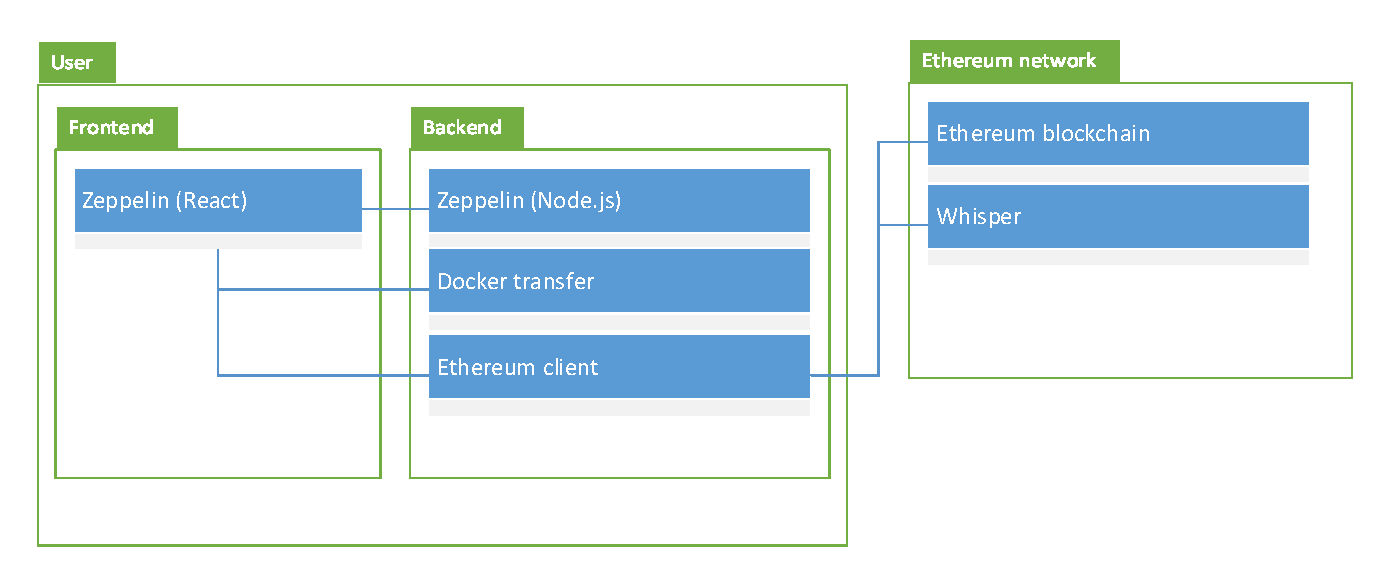
\includegraphics[width=0.80\linewidth, trim=3cm 1cm 3cm 1cm]{figure/deployment.pdf}
\caption{Deployment diagram of Zeppelin}
\end{figure}

\subsection{Contracts}
The Ethereum contract implementation is realized in the C- and JavaScript-like Ethereum-specific language Solidity.
\begin{lstlisting}[caption={WorkAgreement contract}, label={lst:workagreement}]
contract WorkAgreement {
    address client;
    address worker;
    mapping (address => bool) testers;
    uint price;
    uint end;
    function WorkAgreement(address _client, address _worker, uint _price, uint length) {
        client = _client;
        worker = _worker;
        price = _price;
        end = length;
    }
    function addTester(address tester) {
        testers[tester] = true;
    }
}
\end{lstlisting}

\subsection{Security}
The Zeppelin network is resistant to DDoS-attacks, since it is decentralized. Since each user of the network deploys Zeppelin locally, and Ethereum is impervious to DDoS-attacks, service uptime is guaranteed. 

% Skriv om problem vi löser, typ DDoS etc
% UPnP
